\documentclass{standalone}
\usepackage{tikz}
\usetikzlibrary{patterns, positioning}


\begin{document}
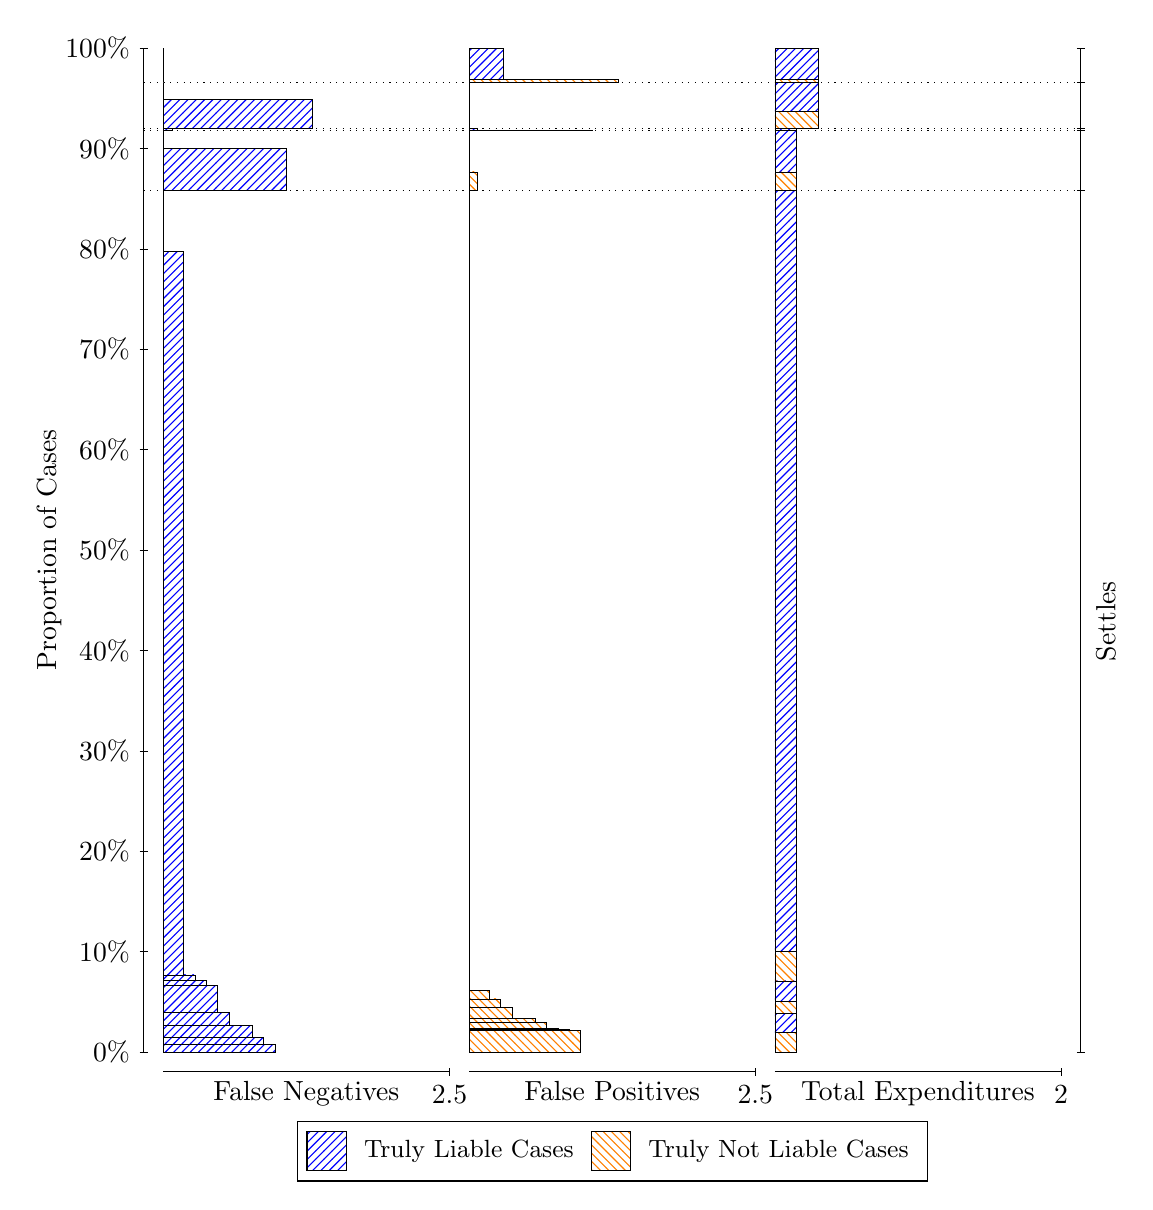
\begin{tikzpicture}
\draw[black, very thin] (1.5,1.75) -- (1.5,14.5);
\node[rotate=90, text=black, anchor=center] at (0.3, 8.125) {Proportion of Cases};
\draw[black, very thin] (1.45,1.75) -- (1.55,1.75);
\node[text=black, anchor=east] at (1.45, 1.75) {0\%};
\draw[black, very thin] (1.45,3.025) -- (1.55,3.025);
\node[text=black, anchor=east] at (1.45, 3.025) {10\%};
\draw[black, very thin] (1.45,4.3) -- (1.55,4.3);
\node[text=black, anchor=east] at (1.45, 4.3) {20\%};
\draw[black, very thin] (1.45,5.575) -- (1.55,5.575);
\node[text=black, anchor=east] at (1.45, 5.575) {30\%};
\draw[black, very thin] (1.45,6.85) -- (1.55,6.85);
\node[text=black, anchor=east] at (1.45, 6.85) {40\%};
\draw[black, very thin] (1.45,8.125) -- (1.55,8.125);
\node[text=black, anchor=east] at (1.45, 8.125) {50\%};
\draw[black, very thin] (1.45,9.4) -- (1.55,9.4);
\node[text=black, anchor=east] at (1.45, 9.4) {60\%};
\draw[black, very thin] (1.45,10.675) -- (1.55,10.675);
\node[text=black, anchor=east] at (1.45, 10.675) {70\%};
\draw[black, very thin] (1.45,11.95) -- (1.55,11.95);
\node[text=black, anchor=east] at (1.45, 11.95) {80\%};
\draw[black, very thin] (1.45,13.225) -- (1.55,13.225);
\node[text=black, anchor=east] at (1.45, 13.225) {90\%};
\draw[black, very thin] (1.45,14.5) -- (1.55,14.5);
\node[text=black, anchor=east] at (1.45, 14.5) {100\%};

\draw[black, very thin] (13.4,1.75) -- (13.4,14.5);
\draw[black, very thin] (13.35,1.75) -- (13.45,1.75);
\node[anchor=west] at (13.35, 1.75) {};
\draw[black, very thin] (13.35,12.693) -- (13.45,12.693);
\node[anchor=west] at (13.35, 12.693) {};
\draw[black, very thin] (13.35,13.455) -- (13.45,13.455);
\node[anchor=west] at (13.35, 13.455) {};
\draw[black, very thin] (13.35,13.479) -- (13.45,13.479);
\node[anchor=west] at (13.35, 13.479) {};
\draw[black, very thin] (13.35,14.064) -- (13.45,14.064);
\node[anchor=west] at (13.35, 14.064) {};
\draw[black, very thin] (13.35,14.5) -- (13.45,14.5);
\node[anchor=west] at (13.35, 14.5) {};

\draw[black, very thin, pattern color=blue, pattern=north east lines] (1.75,1.75) rectangle (3.167,1.843);
\draw[black, very thin, pattern color=blue, pattern=north east lines] (1.75,1.843) rectangle (3.0217,1.935);
\draw[black, very thin, pattern color=blue, pattern=north east lines] (1.75,1.935) rectangle (2.8763,2.0847);
\draw[black, very thin, pattern color=blue, pattern=north east lines] (1.75,2.0847) rectangle (2.731,2.085);
\draw[black, very thin, pattern color=blue, pattern=north east lines] (1.75,2.085) rectangle (2.5857,2.2486);
\draw[black, very thin, pattern color=blue, pattern=north east lines] (1.75,2.2486) rectangle (2.4403,2.5932);
\draw[black, very thin, pattern color=blue, pattern=north east lines] (1.75,2.5932) rectangle (2.295,2.6602);
\draw[black, very thin, pattern color=blue, pattern=north east lines] (1.75,2.6602) rectangle (2.1497,2.73);
\draw[black, very thin, pattern color=blue, pattern=north east lines] (1.75,2.73) rectangle (2.0043,11.913);
\draw[black, very thin, pattern color=orange, pattern=north west lines] (1.75,11.913) rectangle (1.75,12.693);
\draw[black, very thin, pattern color=blue, pattern=north east lines] (1.75,12.693) rectangle (3.3123,13.222);
\draw[black, very thin, pattern color=orange, pattern=north west lines] (1.75,13.222) rectangle (1.75,13.455);
\draw[black, very thin, pattern color=blue, pattern=north east lines] (1.75,13.455) rectangle (1.859,13.477);
\draw[black, very thin, pattern color=orange, pattern=north west lines] (1.75,13.477) rectangle (1.75,13.479);
\draw[black, very thin, pattern color=blue, pattern=north east lines] (1.75,13.479) rectangle (3.6393,13.844);
\draw[black, very thin, pattern color=orange, pattern=north west lines] (1.75,13.844) rectangle (1.75,14.064);
\draw[black, very thin, pattern color=orange, pattern=north west lines] (1.75,14.064) rectangle (1.75,14.104);
\draw[black, very thin, pattern color=blue, pattern=north east lines] (1.75,14.104) rectangle (1.75,14.5);
\draw[black, very thin, pattern color=orange, pattern=north west lines] (5.6333,1.75) rectangle (7.0503,2.027);
\draw[black, very thin, pattern color=orange, pattern=north west lines] (5.6333,2.027) rectangle (6.905,2.0384);
\draw[black, very thin, pattern color=orange, pattern=north west lines] (5.6333,2.0384) rectangle (6.7597,2.0494);
\draw[black, very thin, pattern color=orange, pattern=north west lines] (5.6333,2.0494) rectangle (6.6143,2.1274);
\draw[black, very thin, pattern color=orange, pattern=north west lines] (5.6333,2.1274) rectangle (6.469,2.1758);
\draw[black, very thin, pattern color=orange, pattern=north west lines] (5.6333,2.1758) rectangle (6.3237,2.1758);
\draw[black, very thin, pattern color=orange, pattern=north west lines] (5.6333,2.1758) rectangle (6.3237,2.1759);
\draw[black, very thin, pattern color=orange, pattern=north west lines] (5.6333,2.1759) rectangle (6.1783,2.3208);
\draw[black, very thin, pattern color=orange, pattern=north west lines] (5.6333,2.3208) rectangle (6.033,2.4254);
\draw[black, very thin, pattern color=orange, pattern=north west lines] (5.6333,2.4254) rectangle (5.8877,2.5305);
\draw[black, very thin, pattern color=blue, pattern=north east lines] (5.6333,2.5305) rectangle (5.6333,12.693);
\draw[black, very thin, pattern color=orange, pattern=north west lines] (5.6333,12.693) rectangle (5.7423,12.927);
\draw[black, very thin, pattern color=blue, pattern=north east lines] (5.6333,12.927) rectangle (5.6333,13.455);
\draw[black, very thin, pattern color=orange, pattern=north west lines] (5.6333,13.455) rectangle (7.1957,13.457);
\draw[black, very thin, pattern color=blue, pattern=north east lines] (5.6333,13.457) rectangle (5.7423,13.479);
\draw[black, very thin, pattern color=orange, pattern=north west lines] (5.6333,13.479) rectangle (5.6333,13.699);
\draw[black, very thin, pattern color=blue, pattern=north east lines] (5.6333,13.699) rectangle (5.6333,14.064);
\draw[black, very thin, pattern color=orange, pattern=north west lines] (5.6333,14.064) rectangle (7.5227,14.104);
\draw[black, very thin, pattern color=blue, pattern=north east lines] (5.6333,14.104) rectangle (6.0693,14.5);
\draw[black, very thin, pattern color=orange, pattern=north west lines] (9.5167,1.75) rectangle (9.7892,1.9997);
\draw[black, very thin, pattern color=blue, pattern=north east lines] (9.5167,1.9997) rectangle (9.7892,2.2417);
\draw[black, very thin, pattern color=orange, pattern=north west lines] (9.5167,2.2417) rectangle (9.7892,2.3952);
\draw[black, very thin, pattern color=blue, pattern=north east lines] (9.5167,2.3952) rectangle (9.7892,2.6518);
\draw[black, very thin, pattern color=orange, pattern=north west lines] (9.5167,2.6518) rectangle (9.7892,3.0292);
\draw[black, very thin, pattern color=blue, pattern=north east lines] (9.5167,3.0292) rectangle (9.7892,12.693);
\draw[black, very thin, pattern color=orange, pattern=north west lines] (9.5167,12.693) rectangle (9.7892,12.927);
\draw[black, very thin, pattern color=blue, pattern=north east lines] (9.5167,12.927) rectangle (9.7892,13.455);
\draw[black, very thin, pattern color=orange, pattern=north west lines] (9.5167,13.455) rectangle (9.7892,13.457);
\draw[black, very thin, pattern color=blue, pattern=north east lines] (9.5167,13.457) rectangle (9.7892,13.479);
\draw[black, very thin, pattern color=orange, pattern=north west lines] (9.5167,13.479) rectangle (10.062,13.699);
\draw[black, very thin, pattern color=blue, pattern=north east lines] (9.5167,13.699) rectangle (10.062,14.064);
\draw[black, very thin, pattern color=orange, pattern=north west lines] (9.5167,14.064) rectangle (10.062,14.104);
\draw[black, very thin, pattern color=blue, pattern=north east lines] (9.5167,14.104) rectangle (10.062,14.5);
\draw[black, dotted] (1.5,12.693) -- (13.4,12.693);
\draw[black, dotted] (1.5,13.455) -- (13.4,13.455);
\draw[black, dotted] (1.5,13.479) -- (13.4,13.479);
\draw[black, dotted] (1.5,14.064) -- (13.4,14.064);
\draw[black, very thin] (1.75,1.5) -- (5.3833,1.5);
\node[text=black, anchor=north] at (3.5667, 1.5) {False Negatives};
\draw[black, very thin] (5.3833,1.45) -- (5.3833,1.55);
\node[text=black, anchor=north] at (5.3833, 1.45) {2.5};

\draw[black, very thin] (5.6333,1.5) -- (9.2667,1.5);
\node[text=black, anchor=north] at (7.45, 1.5) {False Positives};
\draw[black, very thin] (9.2667,1.45) -- (9.2667,1.55);
\node[text=black, anchor=north] at (9.2667, 1.45) {2.5};

\draw[black, very thin] (9.5167,1.5) -- (13.15,1.5);
\node[text=black, anchor=north] at (11.333, 1.5) {Total Expenditures};
\draw[black, very thin] (13.15,1.45) -- (13.15,1.55);
\node[text=black, anchor=north] at (13.15, 1.45) {2};

\node[text=black, centered, rotate=90] at (13.72, 7.2217) {Settles};





\draw (7.449999999999999,1.5) node[draw=none] (baseCoordinate) {};
\begin{scope}[align=center]
        \matrix[scale=0.5, draw=black, below=0.5cm of baseCoordinate, nodes={draw}, column sep=0.1cm]{
            \node[rectangle, draw, minimum width=0.5cm, minimum height=0.5cm, pattern color=blue, pattern=north east lines] {}; &
            \node[draw=none, font=\small, text=black] (B) {Truly Liable Cases}; &
            \node[rectangle, draw, minimum width=0.5cm, minimum height=0.5cm, pattern color=orange, pattern=north west lines] {}; &
            \node[draw=none, font=\small, text=black] (B) {Truly Not Liable Cases}; \\
            };
\end{scope}

\end{tikzpicture}
\end{document}